\chapauthor{Орлов М.К.\\Шункевич Д.В.\\Ковалёв М.В.\\Садовский М.Е.\\Загорский А.Г.\\Банцевич К.А.}
\chapter{Комплексная библиотека многократно используемых семантически совместимых компонентов ostis-систем}
\chapauthortoc{Орлов М.К.\\Шункевич Д.В.\\Ковалёв М.В.\\Садовский М.Е.\\Загорский А.Г.\\Банцевич К.А.}
\label{chapter_library}

\begin{scnrelfromlist}{автор}
	\scnitem{Орлов М.К}
\end{scnrelfromlist}

\scntext{тезис}{Всё, что можно сделать одинаково, нужно делать одинаково.}

\scntext{аннотация}{Важнейшим этапом эволюции любой технологии является переход к компонентному проектированию на основе постоянно пополняемой библиотеки многократно используемых компонентов. Идея библиотеки компонентов не нова, но семантическая мощность \textbf{\textit{Библиотеки OSTIS}} значительно выше аналогов за счет того, что подавляющее большинство компонентов библиотеки -- компоненты базы знаний, представленные на унифицированном языке смыслового представления знаний (\textit{SC-коде}). Таким образом, в Библиотеке OSTIS обеспечивается высокий уровень семантической совместимости компонентов, что приводит к высокому уровню семантической совместимости \textit{ostis-систем}, использующих комплексную библиотеку многократно используемых семантически совместимых компонентов ostis-систем.}

\begin{scnrelfromlist}{ключевое понятие}
	\scnitem{компонентное проектирование}
	\scnitem{многократно используемый компонент ostis-систем}
	\scnitem{библиотека многократно используемых компонентов ostis-систем}
	\scnitem{спецификация многократно используемых компонентов ostis-систем} 
	\scnitem{менеджер многократно используемых компонентов ostis-систем}
\end{scnrelfromlist}

\section{Введение в Главу \ref{chapter_library}}

Повторное использование готовых компонентов широко применяется во многих отраслях, связанных с проектированием различного рода систем, поскольку позволяет уменьшить трудоемкость разработки и ее стоимость (путем минимизации количества труда за счет отсутствия необходимости разрабатывать какой-либо компонент), повысить качество создаваемого контента и снизить профессиональные требования к разработчикам компьютерных систем. Таким образом, осуществляется переход от программирования компонентов или целых систем к их дизайну на основе готовых компонентов. Использование готовых компонентов предполагает, что распространяемый компонент верифицирован и документирован, а возможные ошибки и ограничения устранены либо специфицированы и известны.

Рассмотрим проблемы в реализации компонентного подхода к проектированию интеллектуальных систем:
\scncite{Shunkevich2015a}
\begin{SCn}
\scnheader{компонентное проектирование интеллектуальных систем}
\begin{scnrelfromset}{проблемы текущего состояния}
	\scnfileitem{Отсутствие средств \underline{унификации} \underline{любых} видов знаний и моделей представления знаний.}
	\scnfileitem{Отсутствие формальных средств структуризации, позволяющих представить иерархию компонентов на различных уровнях детализации.}
	\scnfileitem{\underline{Несовместимость} компонентов, разработанных в рамках разных проектов, вследствие отсутствия унификации в принципах представления различных видов знаний в рамках одной базы знаний, и, как следствие, отсутствие унификации в принципах выделения и спецификации многократно используемых компонентов.}
	\scnfileitem{Невозможность автоматической интеграции компонентов в систему без ручного вмешательства пользователя.}
	\scnfileitem{Не проводится тестирование, верификация и анализ качества компонентов, не выделяются преимущества, недостатки, ограничения компонентов.}
	\scnfileitem{Не ведётся разработка стандартов, обеспечивающих \underline{совместимость} этих компонентов.}
	\scnfileitem{Многие компоненты используют для идентификации язык разработчика (как правило, английский), и предполагается, что все пользователи будут использовать этот же язык. Однако для многих приложений это недопустимо – понятные только разработчику идентификаторы должны быть скрыты от конечных пользователей, которые должны быть в состоянии выбрать язык для идентификаторов, которые они видят.}
	\scnfileitem{Отсутствие средств поиска компонентов, удовлетворяющих заданных критериям.}
\end{scnrelfromset}
\end{SCn}

Для того, чтобы решить возникшие проблемы, при проектировании интеллектуальных систем и библиотек их многократно используемых компонентов необходимо выполнить следующие требования:
\begin{SCn}
	\scnheader{компонентное проектирование интеллектуальных систем}
	\begin{scnrelfromset}{предъявляемые требования}
		\scnfileitem{Использование \underline{универсального} языка представления знаний, используемого в интеллектуальной системе.}
		\scnfileitem{Наличие универсальной процедуры интеграции знаний в рамках указанного языка.}
		\scnfileitem{Наличие стандарта, обеспечивающего семантическую совместимость интегрируемых знаний (таким стандартом является согласованная система используемых понятий и унифицированная спецификация компонентов).}
	\end{scnrelfromset}
\end{SCn}

Большинство существующих систем создано как автономные программные продукты, которые не могут быть использованы в качестве компонентов других систем. Необходимо использовать либо целую систему, либо ничего. Небольшое число систем поддерживает компонентно-ориентированную архитектуру способную интегрироваться с другими системами \scncite{Iyengar2021} \scncite{Ford2019}. Однако, их интеграция возможна при условии использования одинаковых технологий и только при проектировании одной командой разработчиков \scncite{Donatis2006}.

Многократная повторная разработка уже имеющихся технических решений обусловлена либо тем, что известные технические решения плохо интегрируются в разрабатываемую систему, либо тем, что эти технические решения трудно найти. Данная проблема актуальна как в целом в сфере разработки компьютерных систем, так и в сфере разработки систем, основанных на знаниях, поскольку в системах такого рода степень согласованности различных видов знаний влияет на возможность системы решать нетривиальные задачи.

На данный момент не существует комплексной библиотеки многократно используемых семантически совместимых компонентов компьютерных систем в целом, не говоря об интеллектуальных. Существуют некоторые попытки создания библиотек типовых методов и программ для традиционных компьютерных систем, однако такие библиотеки не решают вышеперечисленные проблемы.

Термин ``библиотека подпрограмм'', одними из первых упомянули Уилкс М., Уиллер Д. и Гилл С. в качестве одной из форм организации вычислений на компьютере (\scncite{Wilkes1951} \scncite{Wilkes1953}). Исходя из изложенного в их книге, под библиотекой понимался набор «коротких, заранее заготовленных программ для отдельных, часто встречающихся (стандартных) вычислительных операций» (\scncite{Volchenskova1984}). Стоит отметить, что компонентами библиотек являются не только программы, но и компоненты интерфейса и базы знаний.

К традиционным решениям относятся \textbf{пакетные менеджеры} языков программирования и операционных систем, а также отдельные системы и платформы с встроенными компонентами и средствами для сохранения создаваемых компонентов.

Компоненты библиотеки могут быть реализованы на разных языках программирования (что приводит к тому, что для каждого языка программирования разрабатываются свои библиотеки со своими решениями различных часто встречаемых ситуаций), а также могут располагаться в разных местах, что приводит к тому, что в библиотеке необходимо средство для поиска компонентов и их установки.

\section{Анализ современных библиотек многократно используемых компонентов}

Современные пакетные менеджеры, такие как npm, pip, poetry, maven, apt, pacman и другие имеют преимущество в том, что они способны разрешать конфликты при установке зависимых компонентов, однако они не учитывают семантику компонентов, а только лишь устанавливают компоненты по идентификатору \scncite{Blahser2021}. Библиотеки таких компонентов являются только лишь хранилищем компонентов, никак не учитывающим назначение компонентов, их преимущества и недостатки, сферы применения, иерархию компонентов и другую информацию, необходимую для интеллектуализации компонентного проектирования компьютерных систем. Поиск компонентов в библиотеках компонентов, соответствующих данных пакетным менеджерам сводится к поиску по идентификатору компонента. Также существенным недостатком современного подхода является платформенная зависимость компонентов. Современные библиотеки компонентов ориентированы только на какой-то определённый язык программирования, операционную систему или платформу.

Пакетный менеджер pip является системой управления пакетами, которая используется для установки пакетов из Python Package Index, который является некоторой библиотекой таких пакетов. Зачастую pip устанавливается вместе с Python. Пакетный менеджер pip используется только для языка программирования Python. 
Он имеет множество функций для работы с пакетами:

\begin{itemize}
	\item установка пакета;
	\item установка пакета специализированной версии;
	\item удаление пакета;
	\item переустановка пакета;
	\item отображение установленных пакетов;
	\item поиск пакетов;
	\item верификация зависимостей пакетов;
	\item создание файла конфигурации со списком установленных пакетов и их версий;
	\item установка множества пакетов из файла конфигурации;
\end{itemize}

\begin{figure}[H]
	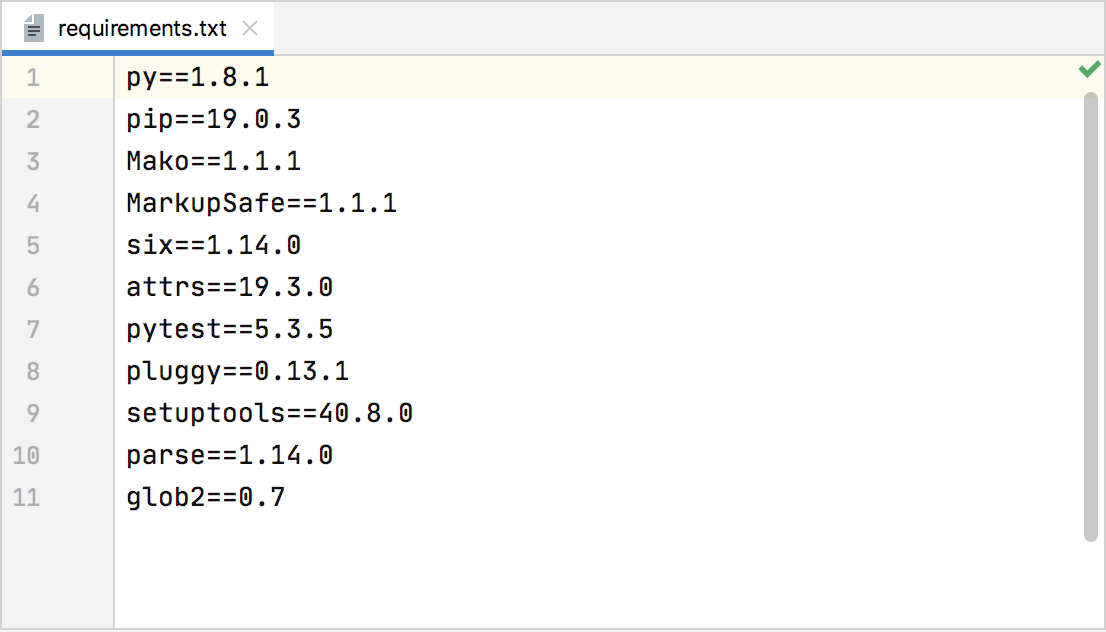
\includegraphics[scale=0.3]{author/part5/figures/pip.png}
	\caption{Файл конфигурации pip}
	\label{fig:pip}
\end{figure}

Пакетный менеджер pip хорошо работает с зависимостями, отображает безуспешно установленные пакеты, а также отображает информацию о требуемой версии пакета при конфликте с другим пакетом.

Альтернативой пакетного менеджера pip является пакетный менеджер poetry, который также ориентирован на язык программирования Python. Преимущество poetry перед pip в том, что он автоматически работает с виртуальными окружениями, способен самостоятельно их находить и создавать. Файл конфигурации для пакетов poetry является более богатым, чем у pip, он хранит такие сведения, как имя проекта, версия проекта, его описание, лицензия, список авторов, URL проекта, его документации и сайта, список ключевых слов проекта и список PyPI классификаторов. Poetry позволяет более гибко настраивать пакеты для проектов Python, файл конфигурации poetry представляет собой более богатую спецификацию проекта, однако эта спецификация не позволяет достичь совместимости между компонентами даже в рамках Python проектов и предназначена преимущественно только для чтения разработчиком. Автоматизировать проектирование компьютерных систем с помощью пакетного менеджера poetry или pip невозможно, так как требуется вмешательство разработчика, который должен вручную совместить интерфейсы устанавливаемых пакетов. Другие пакетные менеджеры языков программирования и операционных систем устроены по такому же принципу: существует хранилище компонентов (библиотека), которая представляет собой множество пакетов этого языка программирования или операционной системы и с которым взаимодействует менеджер компонентов.

\begin{figure}[H]
	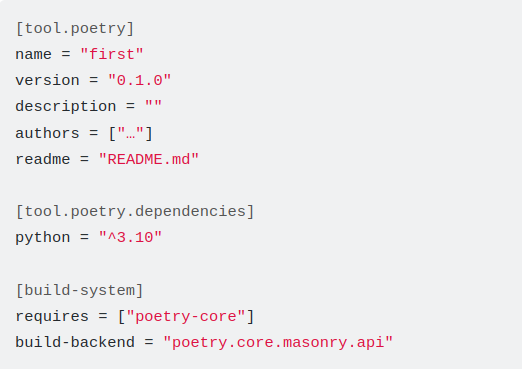
\includegraphics[scale=0.7]{author/part5/figures/poetry.png}
	\caption{Файл конфигурации poetry}
	\label{fig:poetry}
\end{figure}

В качестве компонентного подхода к проектированию программ можно рассмотреть библиотеки подпрограмм современных языков программирования, например, библиотеку стандартных шаблонов С++.

Библиотека стандартных шаблонов -- набор согласованных обобщённых алгоритмов, контейнеров, средств доступа к их содержимому и различных вспомогательных функций в C++.

В библиотеке выделяют пять основных компонентов:
\begin{itemize}
	\item контейнер -- хранение набора объектов в памяти;
	\item итератор -- обеспечение средств доступа к содержимому контейнера;
	\item алгоритм -- определение вычислительной процедуры;
	\item адаптер -- адаптация компонентов для обеспечения различного интерфейса;
	\item функциональный объект — сокрытие функции в объекте для использования другими компонентами.
\end{itemize}

\begin{figure}[H]
	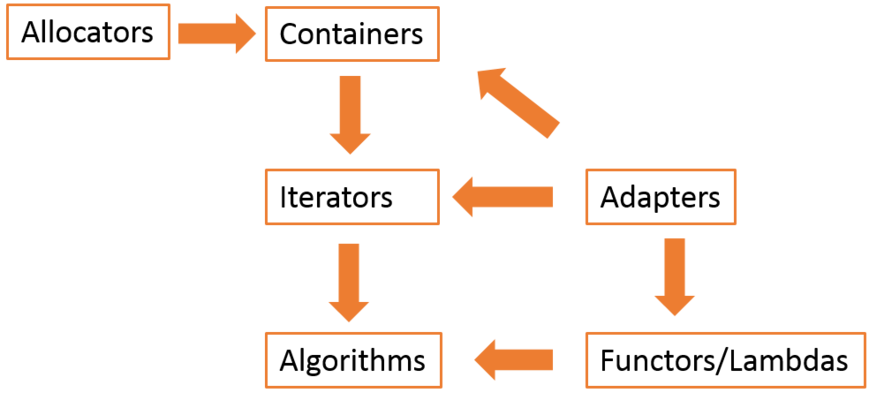
\includegraphics[scale=0.7]{author/part5/figures/STL.png}
	\caption{Структура библиотеки STL}
	\label{fig:STL}
\end{figure}

Разделение позволяет уменьшить количество компонентов. Например, вместо написания отдельной функции поиска элемента для каждого типа контейнера обеспечивается единственная версия, которая работает с каждым из них, пока соблюдаются основные требования.

Совместимость компонентов (контейнеров) в библиотеке стандартных шаблонов обеспечивается общим интерфейсом использования этих компонентов.

Компонентный подход к проектированию компьютерных систем может реализовываться в рамках различных языков, платформ и приложений. Рассмотрим некоторые из них.

% [20] “Modelica StateGraph2”, https://github.com/modelica/Modelica StateGraph2.
На основе языка \textbf{Modelica} разработано большое число свободно-доступных библиотек компонентов, одной из которых является библиотека Modelica\_StateGraph2, включающая компоненты для моделирования дискретных событий, реактивных и гибридных систем с помощью иерархических диаграмм состояния \scncite{Fritzson2014}. Основным недостатком систем на базе языка Modelica является отсутствие совместимости компонентов и достаточной документации, а также узкая направленность разрабатываемых компонентов.

\textbf{Microsoft Power Apps} — это набор приложений, служб и соединителей, а также платформа данных, которая предоставляет среду разработки для эффективного создания пользовательских приложений для бизнеса. Платформа Power Apps имеет средства для создания библиотеки многократно используемых компонентов графического интерфейса, а также предварительно созданные модели распознавания текста (чтение визитных карточек или чеков) и средство обнаружение объектов, которые можно подключить к разрабатываемому приложению \scncite{Prakash2022}. Библиотека компонентов Power Apps представляет собой множество создаваемых пользователем компонентов, которые можно использовать в любых приложениях. Преимущество библиотеки в том, что компоненты могут настраивать свойства по умолчанию, которые можно гибко редактировать в любых приложениях, использующих компоненты. Недостаток в том, что отсутствует семантическая совместимость компонентов, спецификация компонентов, не решена проблема существования семантически эквивалентных компонентов, нету иерархии компонентов и средств поиска этих компонентов. Компоненты платформы Microsoft Power Apps являются многократно используемыми только для однотипных приложений, которые создаются одним и тем же разработчиком.

\textbf{WebProtege} представляет собой многопользовательский веб-интерфейс, позволяющий редактировать и хранить онтологии в формате OWL в совместной среде \scncite{Memduhoglu2018}. Данный проект позволяет не только создавать новые онтологии, но также загружать уже существующие онтологии, которые хранятся на сервере университета Стэнфорда. К преимуществу данного проекта можно отнести автоматическую проверку ошибок в процессе создания объектов онтологий. Данный проект является примером попытки решения проблемы накопления, систематизации и повторного использования уже существующих решений, однако, недостатком данного решения является обособленность разрабатываемых онтологий. Каждый разработанный компонент имеет свою иерархию понятий, подход к выделению классов и сущностей, которые зависят от разработчиков данных онтологий, так как в рамках данного подхода не существует универсальной модели представления знаний, а также формальной спецификации компонентов, представленных в виде онтологий. Следовательно, возникает проблема их семантической несовместимости, что, в свою очередь, приводит к невозможности повторного использования разработанных онтологий при проектировании баз знаний. Данный факт подтверждается наличием на сервере университета Стэнфорда многообразия различных онтологий на одни и те же темы.

\textbf{Платформа IACPaaS} (Intelligent Applications, Control and Platform as a Service)\scncite{Moskalenko2016} – облачная платформа для разработки, управления и удаленного использования интеллектуальных облачных сервисов. Она предназначена для обеспечения поддержки разработки, управления и удаленного использования прикладных и инструментальных мультиагентных облачных сервисов (прежде всего интеллектуальных) и их компонентов для различных предметных областей. Платформа предоставляет доступ:
\begin{itemize}
	\item прикладным пользователям (специалистам в различных предметных областях)(в качестве реализации модели SaaS) - к прикладным сервисам;
	\item разработчикам прикладных и инструментальных сервисов и их компонентов (в качестве реализации модели PaaS) - к инструментальным сервисам;
	\item управляющим интеллектуальными сервисами (в качестве реализации модели Caas);
	\item к сервисам управления.
\end{itemize}

Платформа IACPaaS поддерживает:

\begin{itemize}
	\item базовую технологию разработки прикладных и специализированных инструментальных (интеллектуальных) сервисов с использованием базовыхинструментальных сервисов платформы, поддерживающих эту технологию;
	\item множество специализированных технологий разработки прикладных и специализированных инструментальных (интеллектуальных) сервисов, с использованием специализированных инструментальных сервисов платформы, поддерживающих эти технологии.
\end{itemize}

Платформа IACPaaS также не имеет средств для унифицированного представления компонентов интеллектуальных компьютерных систем и средств для их спецификации и автоматической интеграции.

Исходя из проведённого анализа можно сказать, что на текущем состоянии развития информационных технологий не существует комплексной библиотеки многократно используемых семантически совместимых компонентов компьютерных систем. Таким образом, предлагается комплексная библиотека многократно используемых семантически совместимых компонентов ostis-систем.

\section{Комплексная библиотека многократно используемых семантически совместимых компонентов ostis-систем}

Основным требованием, предъявляемым к \textit{Технологии OSTIS}, является обеспечение возможности совместного использования в рамках ostis-систем различных \textit{видов знаний} и различных \textit{моделей решения задач} с возможностью \underline{неограниченного} расширения перечня используемых в ostis-системе видов знаний и моделей решения задач без существенных трудозатрат, а также различных видов интерфейсов. Следствием данного требования является необходимость реализации компонентного подхода на всех уровнях, от простых компонентов баз знаний, решателей задач и интерфейсов до целых ostis-систем. Разработчики \underline{любой} ostis-системы могут включить в ее состав библиотеку, которая позволит им накапливать и распространять результаты своей деятельности среди других участников \textit{Экосистемы OSTIS} в виде \textbf{\textit{многократно используемых компонентов}}. Решение о включении компонента в библиотеку принимается экспертным сообществом разработчиков, ответственным за качество этой библиотеки. Верификацию компонентов можно автоматизировать.
В рамках \textit{Экосистемы OSTIS} существует множество библиотек многократно используемых компонентов ostis-систем, являющихся подсистемами соответствующих материнских ostis-систем. Материнская ostis-система отвечает за какой-то класс компонентов и является САПРом для этого класса, содержит методики разработки таких компонентов, их классификацию, подробные пояснения ко всем подклассам компонентов. Таким образом, формируется иерархия \textbf{\textit{материнских ostis-систем}}. Материнская ostis-система в свою очередь может являться дочерней ostis-системой для какой-либо другой ostis-системы, заимствуя компоненты из библиотеки, входящей в состав этой другой ostis-системы.

\begin{SCn}
	\scnheader{ostis-система}
	\scnsuperset{материнская ostis-система}
	\begin{scnindent}
		\scnidtf{ostis-система, имеющая в своем составе библиотеку многократно используемых компонентов.}
		\scnhaselement{Метасистема OSTIS}
	\end{scnindent}
	\scnsuperset{дочерняя ostis-система}
	\begin{scnindent}
		\scnidtf{ostis-система, в составе которой имеется компонент, заимствованный из какой-либо библиотеки многократно используемых компонентов.}
	\end{scnindent}
\end{SCn}

Главной библиотекой многократно используемых компонентов ostis-систем является \textit{Библиотека Метасистемы OSTIS}. \textit{Метасистема OSTIS} выступает \textbf{\textit{материнской системой}} для всех разрабатываемых ostis-систем, поскольку содержит все базовые компоненты (рисунок \textit{\nameref{fig:ecosystem_architecture}}).

\begin{figure}[H]
	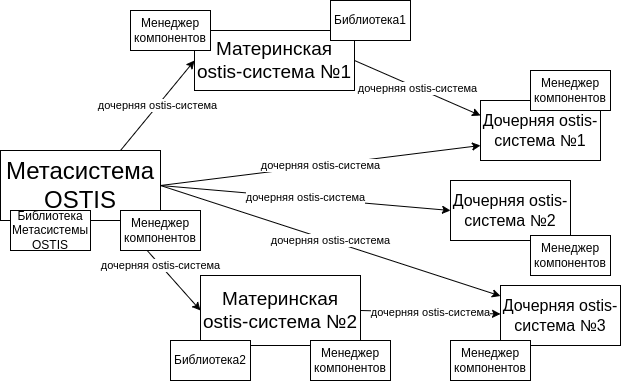
\includegraphics[scale=0.8]{author/part5/figures/ecosystem_architecture.png}
	\caption{Архитектура Экосистемы OSTIS}
	\label{fig:ecosystem_architecture}
\end{figure}

Основу для реализации компонентного подхода в рамках \textit{Технологии OSTIS} составляет \textbf{\textit{Библиотека OSTIS}}. \textit{Метасистема OSTIS} ориентирована на разработку и практическое внедрение методов и средств компонентного проектирования семантически совместимых интеллектуальных систем, которая предоставляет возможность быстрого создания интеллектуальных систем различного назначения. В состав Метасистемы OSTIS входит \textbf{\textit{Библиотека OSTIS}}.
Сферы практического применения технологии компонентного проектирования семантически совместимых интеллектуальных систем ничем не ограничены.

% Понятие ябиблиотеки OSTIS
\begin{SCn}
	\scnheader{библиотека многократно используемых компонентов ostis-систем}
	\scntext{сокращение}{библиотека ostis-систем}
	\scnidtf{библиотека многократно используемых компонентов OSTIS}
	\scnhaselementrole{типичный пример}{\scnkeyword{Библиотека OSTIS}}
	\begin{scnindent}
		\scnidtf{Библиотека многократно используемых компонентов ostis-систем в составе Метасистемы OSTIS}
		\scnidtf{Библиотека Метасистемы OSTIS}
	\end{scnindent}
	\begin{scnreltoset}{объединение}
		\scnitem{библиотека типовых подсистем ostis-систем}
		\scnitem{библиотека шаблонов типовых компонентов ostis-систем}
		\scnitem{библиотека ostis-платформ}
		\scnitem{библиотека многократно используемых компонентов баз знаний}
		\scnitem{библиотека многократно используемых компонентов решателей задач}
		\scnitem{библиотека многократно используемых компонентов пользовательских интерфейсов}
	\end{scnreltoset}
\end{SCn}

% Зачем нужна Библиотека OSTIS
Основное назначение Библиотеки OSTIS -- создание условий для эффективного, осмысленного и массового проектирования ostis-систем и их компонентов путём создания среды для накопления и совместного использования компонентов ostis-систем. Такие условия осуществляются путём неограниченного расширения постоянно эволюционируемых семантически совместимых ostis-систем и их компонентов, входящих в \textit{Экосистему OSTIS}.

Постоянно расширяемая Библиотека OSTIS существенно сокращает сроки разработки новых интеллектуальных компьютерных систем.
библиотека многократно используемых компонентов ostis-систем позволяет избавиться от дублирования семантически эквивалентных информационных компонентов. А также от многообразия форм технической реализации используемых моделей решения задач.

% Что умеет библиотека ostis-систем
Функциональрные возможности библиотеки многократно используемых компонентов ostis-систем:
\begin{SCn}
	\scnheader{библиотека многократно используемых компонентов ostis-систем}
	\begin{scnrelfromset}{функциональные возможности}
		\scnfileitem{Хранение многократно используемых компонентов ostis-систем и их спецификаций. При этом часть компонентов, специфицированных в рамках библиотеки, могут физически храниться в другом месте ввиду особенностей их  технической реализации (например, исходные тексты ostis-платформы могут физически храниться в каком-либо отдельном репозитории, но специфицированы как компонент будут в соответствующей библиотеке). В этом случае спецификация компонента в рамках библиотеки должна также включать описание (1) того \underline{где} располагается компонент и (2) сценария его \underline{автоматической} установки в дочернюю ostis-систему.}
		\scnfileitem{Просмотр имеющихся компонентов и их спецификаций, а также поиск компонентов по фрагментам их спецификации.}
		\scnfileitem{Хранение сведений о том, в каких ostis-системах-потребителях какие из компонентов библиотеки и какой версии используются (были скачаны). Это необходимо как минимум для учета востребованности того или иного компонента, оценки его важности и популярности.}
		\scnfileitem{Систематизация многократно используемых компонентов ostis-систем.}
		\scnfileitem{Обеспечение версионирования многократно используемых компонентов ostis-систем.}
		\scnfileitem{Поиск зависимостей между многократно используемыми компонентами в рамках библиотеки компонентов.}
		\scnfileitem{Формирование отдельных фрагментов многократно используемых компонентов ostis-систем.}
		\scnfileitem{Обеспечение автоматического обновления компонентов, заимствованных в дочерние ostis-системы. Данная функция может включаться и отключаться по желанию разработчиков дочерней ostis-системы. Одновременное обновление одних и тех же компонентов во всех системах, его использующих, не должно \underline{ни в каком контексте} приводить к несогласованности между этими системами. Это требование может оказаться довольно сложным, но без него работа Экосистемы OSTIS невозможна.}
	\end{scnrelfromset}
\end{SCn}

библиотека многократно используемых компонентов ostis-систем является подсистемой ostis-систем, которая имеет свою базу знаний, свой решатель задач и свой интерфейс. Однако не каждая ostis-система обязана иметь библиотеку.

\begin{SCn}
	\scnheader{библиотека многократно используемых компонентов ostis-систем}
	\begin{scnrelfromset}{обобщенная декомпозиция}
		\scnitem{база знаний библиотеки многократно используемых компонентов ostis-систем}
		\scnitem{решатель задач библиотеки многократно используемых компонентов ostis-систем}
		\scnitem{интерфейс библиотеки многократно используемых компонентов ostis-систем}
		\begin{scnindent}
			\begin{scnrelfromset}{декомпозиция}
				\scnitem{минимальный интерфейс библиотеки многократно используемых компонентов ostis-систем}
				\scnitem{расширенный интерфейс библиотеки многократно используемых компонентов ostis-систем}
				\begin{scnindent}
					\scnidtf{графический интерфейс библиотеки многократно используемых компонентов ostis-систем}
				\end{scnindent}
			\end{scnrelfromset}
		\end{scnindent}
	\end{scnrelfromset}
\end{SCn}

решатель задач библиотеки многократно используемых компонентов ostis-систем реализует функциональные возможности библиотеки ostis-систем.

база знаний библиотеки мнoгократно используемых компонентов ostis-систем представляет собой иерархию многократно используемых компонентов ostis-систем и их спецификаций.

интерфейс библиотеки ostis-систем обеспечивает доступ к многократно используемым компонентам и возможностям библиотеки ostis-систем для пользователя и других систем. Существует минимальный и расширенный интерфейс библиотеки многократно используемых компонентов ostis-систем. Минимальный интерфейс позволяет \textit{менеджеру многократно используемых компонентов ostis-систем}, входящему в состав какой-либо дочерней ostis-системы, подключиться к библиотеке многократно используемых компонентов ostis-систем и использовать ее функциональные возможности, то есть, например, получить доступ к спецификации компонентов и установить выбранные компоненты в дочернюю ostis-систему, получить сведения до доступных версиях компонента, его зависимостях и т.д. Расширенный интерфейс, в отличие от минимального интерфейса, позволяет не только получить доступ к компонентам для дальнейшей работы с ними, но и просматривать существующую структуру библиотеки,  а также компоненты и их элементы в удобном и интуитивно понятном для пользователя виде.

% Как происходит интеграция компонентов
Интеграция многократно используемых компонентов ostis-систем сводится к отождествлению ключевых узлов и устранению возможных дублирований и противоречий исходя из спецификации компонента и его содержания. Отождествление sc-элементов происходит в ходе выполнения \textit{действие. отождествить два указанных sc-элемента}, которое рассматривается в главе \ref{chapter_situation_management}. 

Рассмотрим пример интеграции многократно используемого компонента решателя задач, который представляет собой sc-агент поиска кратчайшего пути в графе, в систему управления логистическими процессами. Допустим, система управления логистическими процессами умеет решать задачи, связанные с оптимизацией издержек в процессе создания товара и со складированием товаров. 

\begin{figure}[H]
	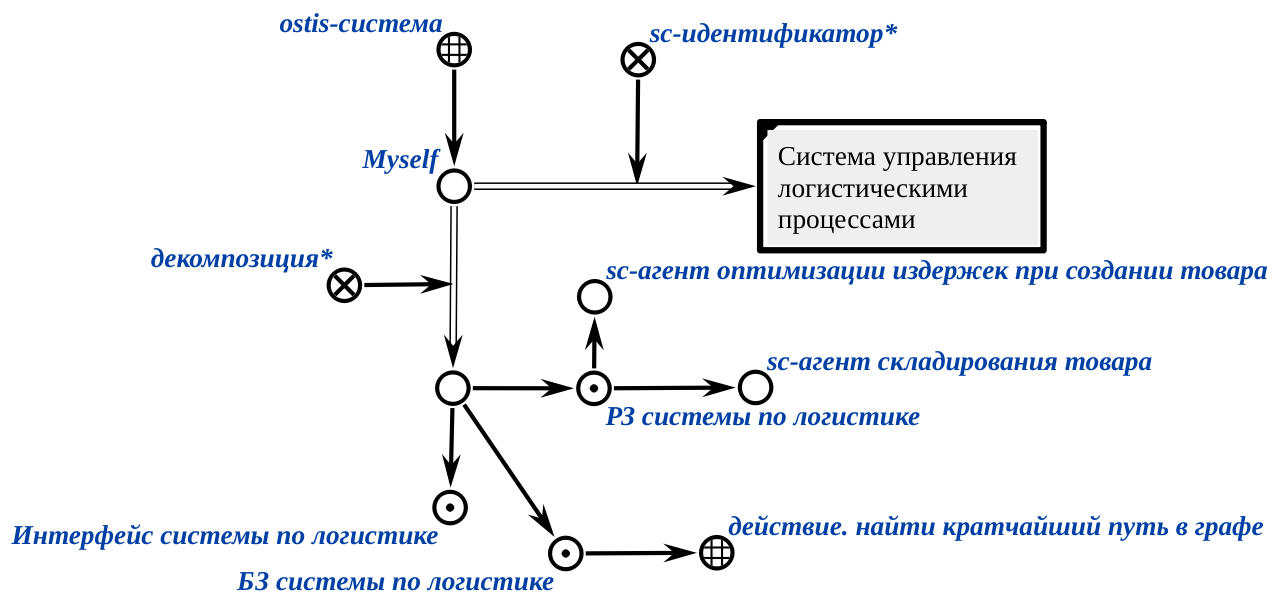
\includegraphics[scale=0.5]{author/part5/figures/logistics_system.png}
	\caption{Структура системы управления логистическими процессами}
	\label{fig:logistics_system}
\end{figure}

При этом в базе знаний системы описано, какие задачи должна решать система и соответствующие им действия. Например, действие. найти кротчайший путь в графе, которое система пока что не умеет выполнять.

Система решения задач по теории графов имеет богатую базу знаний и решатель задач, в том числе имеет sc-агент поиска кратчайшего пути в графе, который специфицирован как многократно используемый компонент и может быть использован в системе по логистике.

\begin{figure}[H]
	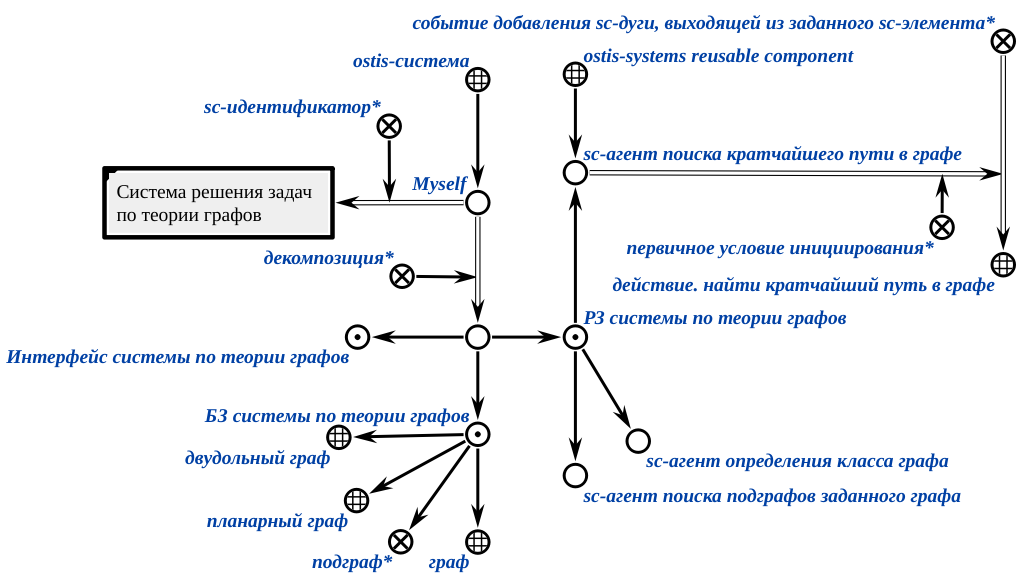
\includegraphics[scale=0.4]{author/part5/figures/graph_theory_system.png}
	\caption{Структура системы решения задач по теории графов}
	\label{fig:graph_theory_system}
\end{figure}

В результате установки многократно используемого компонента в виде sc-агента поиска кратчайшего пути в графе вся его sc-модель погружается в систему решения задач по логистике. При интеграции многократно используемого компонента, который представляет собой sc-агент поиска кратчайшего пути в графе, в систему по логистике ключевой узел \textit{действие. найти кратчайший путь в графе} системы по логистике отождествляется с таким же узлом из установленного компонента из системы по теории графов. Таким образом, при выполнении логистических задач, система сможет интерпретировать действие по поиску кратчайших путей с помощью интегрированного компонента.

Интеграция любых компонентов ostis-систем происходит автоматически, \underline{без} вмешательства разработчика. Это достигается за счёт использования \textit{SC-кода} и его преимуществ, унификации спецификации многократно используемых компонентов и тщательного отбора компонентов в библиотеках экспертным сообществом, ответственным за эту библиотеку.

Рассмотрим понятие многократно используемого компонента ostis-систем. Под многократно используемым компонентом ostis-систем понимается  компонент некоторой ostis-системы, который может быть использован в рамках другой ostis-системы. Это компонент ostis-системы, который может быть использован в других ostis-системах (\textbf{\textit{дочерних ostis-системах}}) и содержит все те и только те sc-элементы, которые необходимы для функционирования компонента в дочерней ostis-системе. Другими словами это компонент некоторой \textbf{\textit{материнской ostis-системы}}, который может быть использован в некоторой дочерней ostis-системе. Многократно используемые компоненты должны иметь унифицированную спецификацию и иерархию для поддержки \underline{совместимости} с другими компонентами. Совместимость многократно используемых компонентов приводит систему к новому качеству, к дополнительному расширению множества решаемых задач при интеграции компонентов.

\begin{SCn}
	\scnheader{многократно используемый компонент ostis-систем}
	\scnidtf{многократно используемый компонент OSTIS}
	\scnidtftext{часто используемый sc-идентификатор}{многократно используемый компонент}
	\scnsubset{компонент ostis-системы}
\end{SCn}

компонент ostis-системы -- это целостная часть ostis-системы, которая содержит все те (и только те) sc-элементы, которые необходимы для её функционирования в ostis-системе.
Отличие многократно используемого компонента ostis-систем от компонента ostis-системы в том, что многократно используемый компонент имеет \underline{спецификацию, достаточную для установки} этого компонента в дочернюю ostis-систему. Спецификация является частью базы знаний библиотеки многократно используемых компонентов соответствующей материнской ostis-системы. Есть техническая возможность встроить многократно используемый компонент в дочернюю ostis-систему.

Требования, предъявляемые к многократно используемым компонентам ostis-систем, наследуют общие требования к проектированию программных компонентов, а также включают следующие:
\begin{itemize}
	\item{Существует техническая возможность встроить многократно используемый компонент в дочернюю ostis-систему.}
	\item{Многократно используемый компонент должен выполнять свои функции наиболее общим образом, чтобы круг возможных систем, в которые он может быть встроен, был наиболее широким.}
	\item{Совместимость многократно используемого компонента: компонент должен стремиться повышать уровень \underline{договороспособности} ostis-систем, в которые он встроен и иметь возможность \underline{автоматической} интеграции в другие системы;}
	\item{Самодостаточность компонентов (или групп компонентов) технологии, т.е. способности их функционировать отдельно от других компонентов без утраты целесообразности их использования.}
\end{itemize}

Рассмотрим классификацию многократно используемых компонентов ostis-систем. Класс многократно используемого компонента ostis-систем является важной частью спецификации компонента, позволяющей лучше понять назначение и область применения данного компонента, а также класс многократно используемого компонента является важнейшим критерием поиска компонентов в библиотеке ostis-систем. Основной признак классификации многократно используемых компонентов является признак предметной области, к которой относится компонент. Здесь структура может быть довольно богатой в соответствии с иерархией областей человеческой деятельности.

\begin{SCn}	
\scnheader{многократно используемый компонент ostis-систем}
\begin{scnrelfromset}{разбиение}
	\scnitem{многократно используемый компонент базы знаний}
	\begin{scnindent}
		\scnsuperset{семантическая окрестность}
		\begin{scnindent}
			\scnhaselement{семантическая окрестность города Минска}
			\scnhaselement{семантическая окрестность понятия множество}
		\end{scnindent}
		\scnsuperset{предметная область и онтология}
		\begin{scnindent}
			\scnhaselement{предметная область и онтология треугольников}
		\end{scnindent}
		\scnsuperset{шаблон типового компонента ostis-систем}
		\begin{scnindent}
			\scnhaselement{Шаблон описания предметной области}
			\scnhaselement{Шаблон описания отношения}
		\end{scnindent}
	\end{scnindent}
	\scnitem{многократно используемый компонент решателя задач}
	\begin{scnindent}
		\scnsuperset{атомарный агент обработки знаний}
		\begin{scnindent}
			\scnhaselement{агент подсчёта мощности множества}
		\end{scnindent}
		\scnsuperset{программа обработки знаний}
	\end{scnindent}
	\scnitem{многократно используемый компонент интерфейса}
	\begin{scnindent}
		\scnsuperset{многократно используемйы компонент пользовательского интерфейса для отображения}
		\scnsuperset{интерактивный многократно используемый компонент пользовательского интерфейса}
	\end{scnindent}
\end{scnrelfromset}
\end{SCn}	

\begin{figure}[H]
	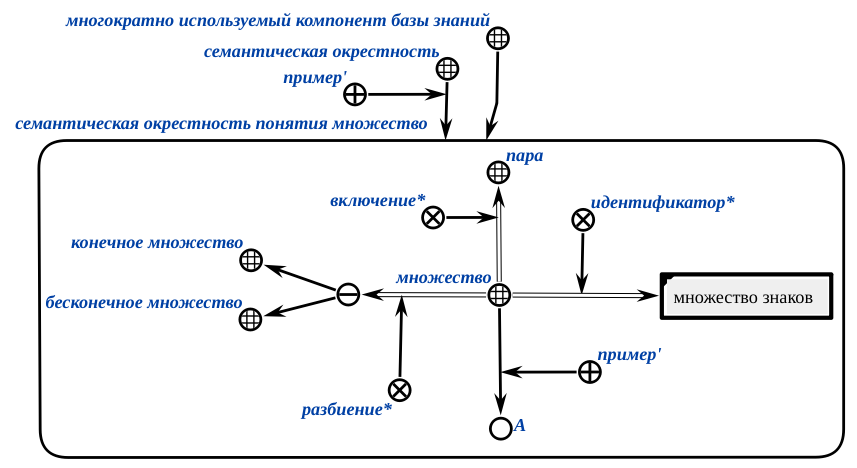
\includegraphics[scale=0.6]{author/part5/figures/set_neighbourhood.png}
	\caption{Пример многократно используемого компонента базы знаний}
	\label{fig:set_neighbourhood}
\end{figure}


Для компонентов баз знаний важнейшим признаком классификации многократно используемых компонентов является \textbf{\textit{вид используемых знаний}}. Для компонентов решателя задач - \textbf{\textit{модель решения задач}}. Для компонентов интерфейса - \textbf{\textit{вид интерфейса}} в соответствии с классификацией компонентов пользовательских интерфейсов.

\begin{SCn}	
\scnheader{многократно используемый компонент ostis-систем}
\scnrelfrom{разбиение}{\scnkeyword{Типология компонентов ostis-систем по атомарности\scnsupergroupsign}}
\begin{scnindent}
	\begin{scneqtoset}
		\scnitem{атомарный многократно используемый компонент ostis-систем}
		\begin{scnindent}
			\scnhaselement{агент подсчёта мощности множества}
		\end{scnindent}
		\scnitem{неатомарный многократно используемый компонент ostis-систем}
		\begin{scnindent}
			\scnhaselement{агент решения геометрических задач}
		\end{scnindent}
	\end{scneqtoset}
\end{scnindent}
\end{SCn}

\textbf{\textit{атомарный многократно используемый компонент ostis-систем}} -- это компонент, который в текущем состоянии библиотеки ostis-систем рассматривается как неделимый, то есть не содержит в своем составе других компонентов. Принадлежность многократно используемого компонента ostis-систем классу атомарных компонентов зависит от того, как специфицирован этот компонент и от существующих на данный момент компонентов в библиотеке. Неатомарный многократно используемый компонент в текущем состоянии библиотеки ostis-систем содержит в своем составе другие атомарные или неатомарные компоненты, он не зависит от своих частей. Без какой-либо части неатомарного компонента его назначение сужается. В общем случае атомарный компонент может перейти в разряд неатомарных в случае, если будет принято решение выделить какую-то из его частей в качестве отдельного компонента. Все вышесказанное, однако, не означает, что даже в случае его платформенной независимости, атомарный компонент всегда хранится в sc-памяти как сформированная sc-структура. Например, платформенно-независимая реализация sc-агента всегда будет представлена набором scp-программ, но будет атомарным многократно используемым компонентом OSTIS в случае, если ни одна из этих программ не будет представлять интереса как самостоятельный компонент. В общем случае неатомарный компонент может перейти в разряд атомарных в случае, если будет принято решение по каким-либо причинам исключить все его части из рассмотрения в качестве отдельных компонентов. Следует отметить, что неатомарный компонент необязательно должен складываться \underline{полностью} из других компонентов, в его состав могут также входить и части, не являющиеся самостоятельными компонентами. Например, в состав реализованного на языке SCP sc-агента, являющего неатомарным многократно используемым компонентом могут входить как scp-программы, которые могут являться многократно используемыми компонентами (а могут и не являться), а также агентная scp-программа, которая не имеет смысла как многократно используемый компонент.

\begin{SCn}	
\scnheader{многократно используемый компонент ostis-систем}
\scnrelfrom{разбиение}{\textbf{\textit{Типология компонентов ostis-систем по зависимости\scnsupergroupsign}}}
\begin{scnindent}
	\begin{scneqtoset}
		\scnitem{зависимый многократно используемый компонент ostis-систем}
		\begin{scnindent}
			\scnhaselement{визуализатор для системы по химии}
		\end{scnindent}
		\scnitem{независимый многократно используемый компонент ostis-систем}
		\begin{scnindent}
			\scnhaselement{предметная область чисел}
		\end{scnindent}
	\end{scneqtoset}
\end{scnindent}
\end{SCn}

\textbf{\textit{зависимый многократно используемый компонент ostis-систем}} зависит хотя бы от одного другого компонента библиотеки ostis-систем, т.е. не может быть встроен в дочернюю ostis-систему без компонентов, от которых он зависит. независимый многократно используемый компонент ostis-систем не зависит ни от одного другого компонента библиотеки ostis-систем.

\begin{SCn}
\scnheader{многократно используемый компонент ostis-систем}
\scnrelfrom{разбиение}{\scnkeyword{Типология компонентов ostis-систем по способу их хранения\scnsupergroupsign}}
\begin{scnindent}
	\begin{scneqtoset}
		\scnitem{многократно используемый компонент ostis-систем, хранящийся в виде внешних файлов}
		\begin{scnindent}
			\begin{scnrelfromset}{разбиение}
				\scnitem{многократно используемый компонент ostis-систем, хранящийся в виде файлов исходных текстов}
				\scnitem{многократно используемый компонент ostis-систем, хранящийся в виде скомпилированных файлов}
			\end{scnrelfromset}
		\end{scnindent}
		\scnitem{многократно используемый компонент, хранящийся в виде sc-структуры}
	\end{scneqtoset}
\end{scnindent}
\end{SCn}

На данном этапе развития \textit{Технологии OSTIS} более удобным является хранение компонентов в виде исходных текстов.

\begin{SCn}
\scnheader{многократно используемый компонент ostis-систем}
\scnrelfrom{разбиение}{\scnkeyword{Типология компонентов ostis-систем по зависимости от ostis-платформы\scnsupergroupsign}}
\begin{scnindent}
	\begin{scneqtoset}
		\scnitem{платформенно-зависимый многократно используемый компонент ostis-систем}
		\begin{scnindent}
			\scnsuperset{ostis-платформа}
			\scnsuperset{абстрактный sc-агент, не реализуемый на Языке SCP}
		\end{scnindent}
		\scnitem{платформенно-независимый многократно используемый компонент ostis-систем}
		\begin{scnindent}
			\scnsuperset{многократно используемый компонент базы знаний}
			\scnsuperset{платформенно-независимый абстрактный sc-агент}
			\scnsuperset{scp-программа}
		\end{scnindent}
	\end{scneqtoset}
\end{scnindent}
\end{SCn}

Под \textbf{\textit{платформенно-зависимым многократно используемым компонентом ostis-систем}} понимается компонент, частично или полностью реализованный при помощи каких-либо сторонних с точки зрения \textit{Технологии OSTIS} средств. Недостаток таких компонентов в том, что интеграция таких компонентов в интеллектуальные системы может сопровождаться дополнительными трудностями, зависящими от конкретных средств реализации компонента. В качестве возможного преимущества платформенно-зависимых многократно используемых компонентов ostis-систем
можно выделить их, как правило, более высокую производительность за счет реализации их на более приближенном к платформе уровне. В общем случае платформенно-зависимый многократно используемый компонент ostis-систем может поставляться как в виде набора исходных кодов, так и скомпилированном виде. Процесс интеграции платформенно-зависимого
многократно используемого компонента ostis-систем в дочернюю систему, разработанную по Технологии OSTIS, сильно зависит от технологий реализации данного компонента и в каждом конкретном случае может состоять из различных этапов. Каждый платформенно-зависимый многократно используемый компонент ostis-систем должен иметь соответствующую подробную, корректную и понятную инструкцию по его установке и внедрению в дочернюю систему.
Под \textbf{\textit{платформенно-независимым многократно используемым компонентом ostis-систем}} понимается компонент, который целиком и полностью представлен на \textit{SC-коде}. В случае неатомарного многократно используемого компонента это означает, что все более простые компоненты, входящие в его состав также обязаны быть платформенно-независимыми многократно используемыми компонентами ostis-систем. Процесс интеграции платформенно-зависимого многократно используемого компонента ostis-систем в дочернюю систему, разработанную по Технологии OSTIS, существенно упрощается за счет использования общей унифицированной
формальной основы представления и обработки знаний.

Наиболее ценными являются платформенно-независимые многократно используемые компоненты ostis-систем.

\begin{SCn}
\scnheader{многократно используемый компонент ostis-систем}
\scnrelfrom{разбиение}{\scnkeyword{Типология компонентов ostis-систем по динамичности их установки\scnsupergroupsign}}
\begin{scnindent}
	\begin{scneqtoset}
		\scnitem{динамически устанавливаемый многократно используемый компонент ostis-систем}
		\begin{scnindent}
			\scnidtf{многократно используемый компонент, при установке которого система не требует перезапуска}
			\begin{scnrelfromset}{декомпозиция}
				\scnitem{многократно используемый компонент, хранящийся в виде скомпилированных файлов}
				\scnitem{многократно используемый компонент базы знаний}
			\end{scnrelfromset}
		\end{scnindent}
		\scnitem{многократно используемый компонент, при установке которого система требует перезапуска}
	\end{scneqtoset}
\end{scnindent}
\end{SCn}

Процесс интеграции компонентов разных видов на разных этапах жизненного цикла osits-систем бывает разным. Наиболее ценными являются компоненты, которые могут быть интегрированы в работающую систему \underline{без} прекращения её функционирования. Некоторые системы, особенно системы управления, нельзя останавливать, а устанавливать и обновлять компоненты нужно.

\begin{SCn}
\scnheader{многократно используемый компонент ostis-систем}
\scnsuperset{типовая подсистема ostis-систем}
\begin{scnindent}
	\scnhaselement{Среда коллективной разработки баз знаний ostis-систем}
	\scnhaselement{Визуальный web-ориентированный редактор sc.g-текстов}
\end{scnindent}
\end{SCn}

Для того, чтобы хранить многократно используеме компоненты ostis-систем, необходимо некоторое хранилище. Таким хранилищем может выступать как какая-либо ostis-система, так и сторонее хранилище, например, облачный сервис. Помимо внешних файлов компонента в хранилище должна находиться его \underline{спецификация}.

Каждый \textit{многократно используемый компонент ostis-систем} должен быть специфицирован в рамках библиотеки. Данные спецификации включают в себя основные знания о компоненте, которые позволяют обеспечить построение полной иерархии компонентов и их зависимостей, а также обеспечивают \underline{беспрепятственную} интеграцию компонентов в дочерние ostis-системы. Для спецификации компонента используеются, как отношения, так и классы компонента.

Чтобы многократно используемый компонент мог быть принят в библиотеку, нужно специфицировать его используя \textit{необходимое для установки отношение, специфицирующее многократно используемый компонент ostis-систем}. В то же время \textit{необязательное для установки отношение, специфицирующее многократно используемый компонент ostis-систем} помогает лучше понять суть компонента, упрощает поиск, но не является обязательным для того, чтобы компонент мог быть установлен в ostis-систему.

\begin{SCn}
\scnheader{отношение, специфицирующее многократно используемый компонент ostis-систем\scnsupergroupsign}
\scnidtf{отношение, которое используется при спецификации многократно используемого компонента ostis-систем}
\begin{scnrelfromset}{разбиение}
	\scnitem{необходимое для установки отношение, специфицирующее многократно используемый компонент ostis-систем}
	\begin{scnindent}
		\scnhaselement{метод установки*}
		\scnhaselement{адрес хранилища*}
		\scnhaselement{зависимости компонента*}
	\end{scnindent}
	\scnitem{необязательное для установки отношение, специфицирующее многократно используемый компонент ostis-систем}
	\begin{scnindent}
		\scnhaselement{сопутствующий компонент*}
		\scnhaselement{история изменений*}
		\scnhaselement{авторы*}
		\scnhaselement{примечание*}
		\scnhaselement{пояснение*}
		\scnhaselement{идентификатор*}
		\scnhaselement{ключевой sc-элемент*}
		\scnhaselement{назначение*}
	\end{scnindent}
\end{scnrelfromset}
\end{SCn}

Метод установки позволяет пользователю установить компонент вручную, а \textbf{\textit{менеджеру компонентов}} - автоматически. Основные два метода установки многократно используемых компонентов - метод установки динамически устанавливаемого многократно используемого компонента ostis-систем и метод установки многократно используемого компонента, при установке которого система требует перезапуска. При динамической установке необходимо только скачать компонент, и он сразу же функционирует в системе. 

\begin{figure}[H]
	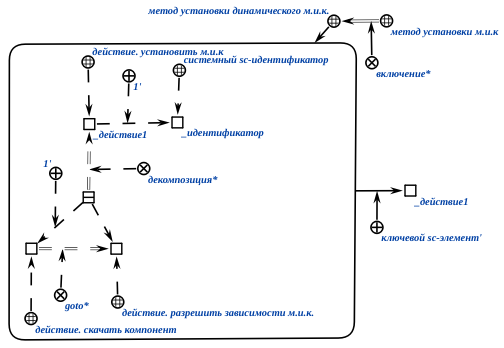
\includegraphics[scale=0.8]{author/part5/figures/install_dynamic_method.png}
	\caption{Метод установки динамически устанавливаемого многократно используемого компонента ostis-систем}
	\label{fig:dynamic_method}
\end{figure}

При установке компонента, при установке которого система требует перезапуска необходимо помимо скачивания компонента транслировать его в память системы.

\begin{figure}[H]
	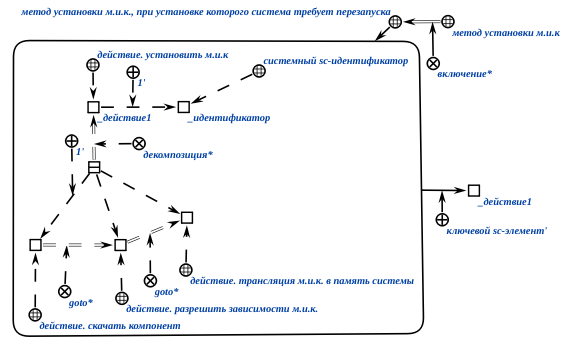
\includegraphics[scale=0.8]{author/part5/figures/install_with_reboot_method.png}
	\caption{Метод установки динамически устанавливаемого многократно используемого компонента, при установке которого система требует перезапуска}
	\label{fig:install_with_reboot_method}
\end{figure}


Связки отношения \textit{адрес хранилища*} связывают многократно используемый компонент, хранящийся в виде внешних файлов и файл, содержащий url-адрес многократно используемого компонента ostis-систем. Таким файлом может быть файл, содержащий url-адрес на GitHub многократно используемого компонента ostis-систем, файл, содержащий url-адрес на Google Drive многократно используемого компонента ostis-систем, файл, содержащий url-адрес на Docker Hub многократно используемого компонента ostis-систем и другие.

Связки отношения \textit{зависимости компонента*} связывают многократно используемый компонент, и множество компонентов, без которых устанавливаемый компонент \underline{не может быть} встроен в дочернюю ostis-систему.

\begin{figure}[H]
	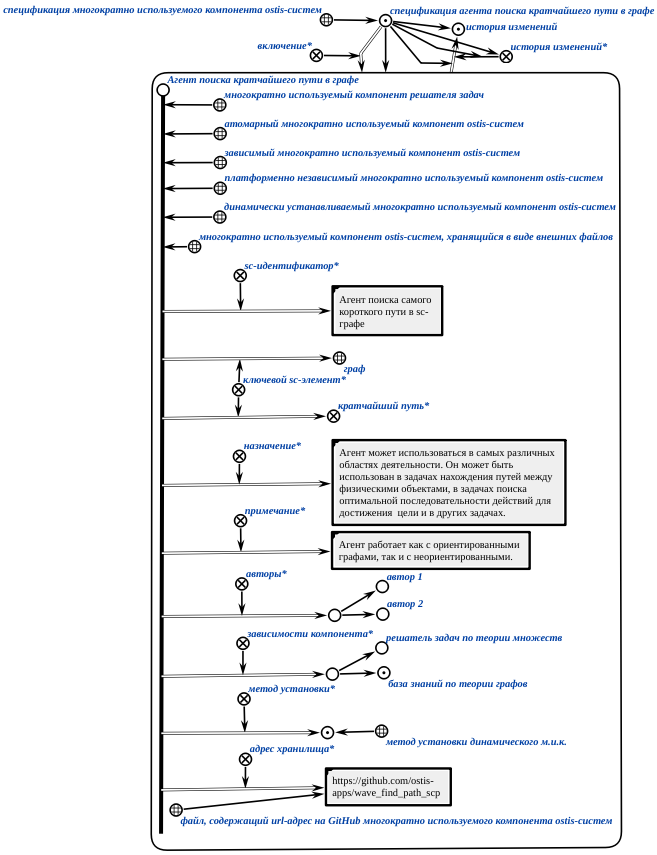
\includegraphics[scale=0.6]{author/part5/figures/component_specification_example.png}
	\caption{Пример спецификации многократно используемого компонента ostis-систем}
	\label{fig:component_specification_example}
\end{figure}

В некоторых случаях может оказаться, что для использования одного многократно используемого компонента OSTIS целесообразно или даже необходимо дополнительно использовать несколько других многократно используемых компонентов OSTIS. Например, может оказаться целесообразным вместе с каким либо sc-агентом информационного поиска использовать соответствующую команду интерфейса, которая представлена отдельным
компонентом и позволит пользователю задавать вопрос для указанного sc-агента через интерфейс системы. В таких случаях для связи компонентов используется отношение \textit{сопутствующий компонент*}. Наличие таких связей позволяет устранить возможные проблемы неполноты знаний и навыков в дочерней системе, из-за которых какие-либо из компонентов могут не выполнять свои функции. Связки отношения сопутствующий компонент* связывают многократно используемые компоненты ostis-систем, которые целесообразно использовать в дочерней системе вместе. Каждая такая связка может дополнительно быть снабжена sc-комментарием или sc-пояснением, отражающим суть указываемой зависимости.

\section{Менеджер многократно используемых компонентов ostis-систем}

менеджер многократно используемых компонентов ostis-систем -- подсистема ostis-системы, с помощью которой проиходит взаимодействие с библиотекой компонентов ostis-систем.

\begin{SCn}
\scnheader{менеджер многократно используемых компонентов ostis-систем}
\scnidtftext{часто используемый sc-идентификатор}{менеджер многократно используемых компонентов}
\scnidtftext{часто используемый sc-идентификатор}{менеджер компонентов}
\begin{scnrelfromset}{обобщенная декомпозиция}
	\scnitem{база знаний менеджера многократно используемых компонентов ostis-систем}
	\scnitem{решатель задач менеджера многократно используемых компонентов ostis-систем}
	\scnitem{интерфейс менеджера многократно используемых компонентов ostis-систем}
\end{scnrelfromset}
\end{SCn}

База знаний менеджера компонентов содержит все те знания, которые необходимы для установки многократно используемого компонента в дочернюю ostis-систему. К таким знаниям относятся знания о спецификации многократно используемых компонентов, методы установки компонентов, знание о  библиотеках ostis-систем, с которыми происходит взаимодействие. Решатель задач менеджера компонентов взаимодействует с библиотекой ostis-систем и позволяет установить и интегрировать многократно используемые компоненты в дочернюю ostis-систему, также выполнять поиск, обновление, публикацию, удаление компонентов. Интерфейс менеджера многократно используемых компонентов обеспечивает удобное для пользователя и других систем использование менеджера компонентов.

Функциональные возможности менеджера компонентов ostis-систем следующие:
\begin{itemize}
	\item{\textbf{Поиск многократно используемых компонентов ostis-систем}. Множество возможных критериев поиска соответствует спецификации многократно используемых компонентов. Такими критериями могут быть классы компонента, его авторы, идентификатор, фрагмент примечания, назначение, принадлежность какой-либо предметной области, вид знаний компонента и другие.}
	\item{\textbf{Установка многократно используемого компонента ostis-систем}. Установка многократно используемого компонента происходит вне зависимости от типологии, способа установки и местоположения компонента. Необходимое условие для возможности установки многократно используемого компонента -- наличие \textbf{\textit{спецификации многократно используемого компонента ostis-систем}}. Перед установкой многократно используемого компонента в дочернюю систему необходимо разрешить все зависимости путём установки зависимых компонентов. После успешной установки компонента, в базе знаний дочерней системы генерируется информационная конструкция, обозначающая факт установки компонента в систему с помощью отношения \textit{установленные компоненты*}. После установки компонента в ostis-систему могут возникнуть противоречия в базе знаний, которые  устраняются с помощью средств обнаружения и анализа ошибок и противоречий в базе знаний ostis-системы.}
	\item{\textbf{Публикация многократно используемого компонента ostis-систем в библиотеку ostis-систем}. При публикации компонента в библиотеку ostis-систем происходит верификация на основе спецификации компонента. Также существует возможность обновления версии опубликованного компонента сообществом его разработчиков.}
	\item{\textbf{Обновление установленного многократно используемого компонента ostis-систем}}
	\item{\textbf{Удаление установленного многократно используемого компонента}. Как и в случае установки после удаления многократно используемого компонента из ostis-системы в базе знаний системы устанавливается факт удаления компонента. Эта информация является важной частью \underline{истории эксплуатации} ostis-системы.}
	\item{\textbf{Добавление и удаление отслеживаемых ostis-системой библиотек}. Менеджер компонентов содержит информацию о множестве источников для установки компонентов, перечень которых можно дополнять вручную. По умолчанию менеджер компонентов отслеживает Библиотеку Метасистемы OSTIS, однако можно создавать и добавлять дополнительные библиотеки ostis-систем.}
\end{itemize}

\section{Многократно используемые компоненты баз знаний ostis-систем}

На сегодняшний день разработано большое число \textit{баз знаний} по самым различным предметным областям. Однако в большинстве случаев каждая база знаний разрабатывается отдельно и независимо от других, в отсутствие единой унифицированной формальной основы для представления знаний, а также единых принципов формирования систем понятий для описываемой предметной области. В связи с этим разработанные базы оказываются, как правило, несовместимы между собой и не пригодны для повторного использования. Компонентный подход к разработке интеллектуальных компьютерных систем, реализуемый в виде \textbf{\textit{библиотеки многократно используемых компонентов ostis-систем}}, позволяет решить описанные проблемы.

\section{Многократно используемые встраиваемые ostis-системы}

%%%%%%%%%%%%%%%%%%%%%%%%% referenc.tex %%%%%%%%%%%%%%%%%%%%%%%%%%%%%%
% sample references
% %
% Use this file as a template for your own input.
%
%%%%%%%%%%%%%%%%%%%%%%%% Springer-Verlag %%%%%%%%%%%%%%%%%%%%%%%%%%
%
% BibTeX users please use
% \bibliographystyle{}
% \bibliography{}
%
\biblstarthook{In view of the parallel print and (chapter-wise) online publication of your book at \url{www.springerlink.com} it has been decided that -- as a genreral rule --  references should be sorted chapter-wise and placed at the end of the individual chapters. However, upon agreement with your contact at Springer you may list your references in a single seperate chapter at the end of your book. Deactivate the class option \texttt{sectrefs} and the \texttt{thebibliography} environment will be put out as a chapter of its own.\\\indent
References may be \textit{cited} in the text either by number (preferred) or by author/year.\footnote{Make sure that all references from the list are cited in the text. Those not cited should be moved to a separate \textit{Further Reading} section or chapter.} If the citatiion in the text is numbered, the reference list should be arranged in ascending order. If the citation in the text is author/year, the reference list should be \textit{sorted} alphabetically and if there are several works by the same author, the following order should be used:
\begin{enumerate}
\item all works by the author alone, ordered chronologically by year of publication
\item all works by the author with a coauthor, ordered alphabetically by coauthor
\item all works by the author with several coauthors, ordered chronologically by year of publication.
\end{enumerate}
The \textit{styling} of references\footnote{Always use the standard abbreviation of a journal's name according to the ISSN \textit{List of Title Word Abbreviations}, see \url{http://www.issn.org/en/node/344}} depends on the subject of your book:
\begin{itemize}
\item The \textit{two} recommended styles for references in books on \textit{mathematical, physical, statistical and computer sciences} are depicted in ~\cite{science-contrib, science-online, science-mono, science-journal, science-DOI} and ~\cite{phys-online, phys-mono, phys-journal, phys-DOI, phys-contrib}.
\item Examples of the most commonly used reference style in books on \textit{Psychology, Social Sciences} are~\cite{psysoc-mono, psysoc-online,psysoc-journal, psysoc-contrib, psysoc-DOI}.
\item Examples for references in books on \textit{Humanities, Linguistics, Philosophy} are~\cite{humlinphil-journal, humlinphil-contrib, humlinphil-mono, humlinphil-online, humlinphil-DOI}.
\item Examples of the basic Springer style used in publications on a wide range of subjects such as \textit{Computer Science, Economics, Engineering, Geosciences, Life Sciences, Medicine, Biomedicine} are ~\cite{basic-contrib, basic-online, basic-journal, basic-DOI, basic-mono}. 
\end{itemize}
}

\begin{thebibliography}{99.}%
% and use \bibitem to create references.
%
% Use the following syntax and markup for your references if 
% the subject of your book is from the field 
% "Mathematics, Physics, Statistics, Computer Science"
%
% Contribution 
\bibitem{science-contrib} Broy, M.: Software engineering --- from auxiliary to key technologies. In: Broy, M., Dener, E. (eds.) Software Pioneers, pp. 10-13. Springer, Heidelberg (2002)
%
% Online Document
\bibitem{science-online} Dod, J.: Effective substances. In: The Dictionary of Substances and Their Effects. Royal Society of Chemistry (1999) Available via DIALOG. \\
\url{http://www.rsc.org/dose/title of subordinate document. Cited 15 Jan 1999}
%
% Monograph
\bibitem{science-mono} Geddes, K.O., Czapor, S.R., Labahn, G.: Algorithms for Computer Algebra. Kluwer, Boston (1992) 
%
% Journal article
\bibitem{science-journal} Hamburger, C.: Quasimonotonicity, regularity and duality for nonlinear systems of partial differential equations. Ann. Mat. Pura. Appl. \textbf{169}, 321--354 (1995)
%
% Journal article by DOI
\bibitem{science-DOI} Slifka, M.K., Whitton, J.L.: Clinical implications of dysregulated cytokine production. J. Mol. Med. (2000) doi: 10.1007/s001090000086 
%
\bigskip

% Use the following (APS) syntax and markup for your references if 
% the subject of your book is from the field 
% "Mathematics, Physics, Statistics, Computer Science"
%
% Online Document
\bibitem{phys-online} J. Dod, in \textit{The Dictionary of Substances and Their Effects}, Royal Society of Chemistry. (Available via DIALOG, 1999), 
\url{http://www.rsc.org/dose/title of subordinate document. Cited 15 Jan 1999}
%
% Monograph
\bibitem{phys-mono} H. Ibach, H. L\"uth, \textit{Solid-State Physics}, 2nd edn. (Springer, New York, 1996), pp. 45-56 
%
% Journal article
\bibitem{phys-journal} S. Preuss, A. Demchuk Jr., M. Stuke, Appl. Phys. A \textbf{61}
%
% Journal article by DOI
\bibitem{phys-DOI} M.K. Slifka, J.L. Whitton, J. Mol. Med., doi: 10.1007/s001090000086
%
% Contribution 
\bibitem{phys-contrib} S.E. Smith, in \textit{Neuromuscular Junction}, ed. by E. Zaimis. Handbook of Experimental Pharmacology, vol 42 (Springer, Heidelberg, 1976), p. 593
%
\bigskip
%
% Use the following syntax and markup for your references if 
% the subject of your book is from the field 
% "Psychology, Social Sciences"
%
%
% Monograph
\bibitem{psysoc-mono} Calfee, R.~C., \& Valencia, R.~R. (1991). \textit{APA guide to preparing manuscripts for journal publication.} Washington, DC: American Psychological Association.
%
% Online Document
\bibitem{psysoc-online} Dod, J. (1999). Effective substances. In: The dictionary of substances and their effects. Royal Society of Chemistry. Available via DIALOG. \\
\url{http://www.rsc.org/dose/Effective substances.} Cited 15 Jan 1999.
%
% Journal article
\bibitem{psysoc-journal} Harris, M., Karper, E., Stacks, G., Hoffman, D., DeNiro, R., Cruz, P., et al. (2001). Writing labs and the Hollywood connection. \textit{J Film} Writing, 44(3), 213--245.
%
% Contribution 
\bibitem{psysoc-contrib} O'Neil, J.~M., \& Egan, J. (1992). Men's and women's gender role journeys: Metaphor for healing, transition, and transformation. In B.~R. Wainrig (Ed.), \textit{Gender issues across the life cycle} (pp. 107--123). New York: Springer.
%
% Journal article by DOI
\bibitem{psysoc-DOI}Kreger, M., Brindis, C.D., Manuel, D.M., Sassoubre, L. (2007). Lessons learned in systems change initiatives: benchmarks and indicators. \textit{American Journal of Community Psychology}, doi: 10.1007/s10464-007-9108-14.
%
%
% Use the following syntax and markup for your references if 
% the subject of your book is from the field 
% "Humanities, Linguistics, Philosophy"
%
\bigskip
%
% Journal article
\bibitem{humlinphil-journal} Alber John, Daniel C. O'Connell, and Sabine Kowal. 2002. Personal perspective in TV interviews. \textit{Pragmatics} 12:257--271
%
% Contribution 
\bibitem{humlinphil-contrib} Cameron, Deborah. 1997. Theoretical debates in feminist linguistics: Questions of sex and gender. In \textit{Gender and discourse}, ed. Ruth Wodak, 99--119. London: Sage Publications.
%
% Monograph
\bibitem{humlinphil-mono} Cameron, Deborah. 1985. \textit{Feminism and linguistic theory.} New York: St. Martin's Press.
%
% Online Document
\bibitem{humlinphil-online} Dod, Jake. 1999. Effective substances. In: The dictionary of substances and their effects. Royal Society of Chemistry. Available via DIALOG. \\
http://www.rsc.org/dose/title of subordinate document. Cited 15 Jan 1999
%
% Journal article by DOI
\bibitem{humlinphil-DOI} Suleiman, Camelia, Daniel C. O'Connell, and Sabine Kowal. 2002. `If you and I, if we, in this later day, lose that sacred fire...': Perspective in political interviews. \textit{Journal of Psycholinguistic Research}. doi: 10.1023/A:1015592129296.
%
%
%
\bigskip
%
%
% Use the following syntax and markup for your references if 
% the subject of your book is from the field 
% "Computer Science, Economics, Engineering, Geosciences, Life Sciences"
%
%
% Contribution 
\bibitem{basic-contrib} Brown B, Aaron M (2001) The politics of nature. In: Smith J (ed) The rise of modern genomics, 3rd edn. Wiley, New York 
%
% Online Document
\bibitem{basic-online} Dod J (1999) Effective Substances. In: The dictionary of substances and their effects. Royal Society of Chemistry. Available via DIALOG. \\
\url{http://www.rsc.org/dose/title of subordinate document. Cited 15 Jan 1999}
%
% Journal article by DOI
\bibitem{basic-DOI} Slifka MK, Whitton JL (2000) Clinical implications of dysregulated cytokine production. J Mol Med, doi: 10.1007/s001090000086
%
% Journal article
\bibitem{basic-journal} Smith J, Jones M Jr, Houghton L et al (1999) Future of health insurance. N Engl J Med 965:325--329
%
% Monograph
\bibitem{basic-mono} South J, Blass B (2001) The future of modern genomics. Blackwell, London 
%
\end{thebibliography}
